\documentclass[a4paper, 11pt]{article}

%Comandos para configurar el idioma
\usepackage[spanish,activeacute]{babel}
\usepackage[utf8]{inputenc}
\usepackage[T1]{fontenc} %Necesario para el uso de las comillas latinas.
\usepackage{geometry}
\usepackage{graphicx}

% Bibliografía
\usepackage{babelbib}
\usepackage[nottoc,notlot,notlof]{tocbibind}

%Importante que esta sea la última órden del preámbulo
\usepackage{hyperref}

\newcommand\fnurl[2]{%
\href{#2}{#1}\footnote{\url{#2}}%
}

\newcommand{\includecode}[2][c]{\lstinputlisting[caption=#2, escapechar=, style=custom#1]{#2}<!---->}

%Paquetes matemáticos
\usepackage{amsmath,amsfonts,amsthm}
\usepackage[all]{xy} %Para diagramas
\usepackage{enumerate} %Personalización de enumeraciones
\usepackage{tikz} %Dibujos

%Tipografía escalable
\usepackage{lmodern}
%Legibilidad
\usepackage{microtype}

%Código
\usepackage{listings}
\usepackage{color}

\definecolor{dkgreen}{rgb}{0,0.6,0}
\definecolor{gray}{rgb}{0.5,0.5,0.5}
\definecolor{mauve}{rgb}{0.58,0,0.82}

\definecolor{listinggray}{gray}{0.9}
\definecolor{lbcolor}{rgb}{0.9,0.9,0.9}
\lstset{
    backgroundcolor=\color{lbcolor},
    tabsize=4,
    rulecolor=,
    language=[GNU]C++,
    basicstyle=\scriptsize,
    upquote=true,
    aboveskip={1.5\baselineskip},
    columns=fixed,
    showstringspaces=false,
    extendedchars=false,
    breaklines=true,
    prebreak = \raisebox{0ex}[0ex][0ex]{\ensuremath{\hookleftarrow}},
    frame=single,
    numbers=left,
    showtabs=false,
    showspaces=false,
    showstringspaces=false,
    identifierstyle=\ttfamily,
    keywordstyle=\color[rgb]{0,0,1},
    commentstyle=\color[rgb]{0.026,0.112,0.095},
    stringstyle=\color[rgb]{0.627,0.126,0.941},
    numberstyle=\color[rgb]{0.205, 0.142, 0.73
%   \lstdefinestyle{C++}{language=C++,style=numbers}’.
}
\{
    backgroundcolor=\color{lbcolor},
    tabsize=4,
    language=C++,
    captionpos=b,
    tabsize=3,
    frame=lines,
    numbers=left,
    numberstyle=\tiny,
    numbersep=5pt,
    breaklines=true,
    showstringspaces=false,
    basicstyle=\footnotesize,
    %  identifierstyle=\color{magenta},
    keywordstyle=\color[rgb]{0,0,1},
    commentstyle=\color[rgb]{0.026,0.112,0.095}, % Darkgreen
    stringstyle=\color{red},
    escapeinside={(*@}{@*)}
}
% Slightly bigger margins than the latex defaults

\geometry{verbose,tmargin=1in,bmargin=1in,lmargin=1in,rmargin=1in}
\setlength{\parskip}{.5em} % por defecto el espacio entre párrafos es 0pt

\theoremstyle{definition}
\newtheorem{ejercicio}{Ejercicio}
\newtheorem{cuestion}{Cuestión}
\newtheorem*{solucion}{Solución}
\newtheorem*{bonus}{BONUS}

%%%%%%%% New sqrt
\usepackage{letltxmacro}
\makeatletter
\let\oldr@@t\r@@t
\def\r@@t#1#2{%
\setbox0=\hbox{$\oldr@@t#1{#2\,}$}\dimen0=\ht0
\advance\dimen0-0.2\ht0
\setbox2=\hbox{\vrule height\ht0 depth -\dimen0}%
{\box0\lower0.4pt\box2}}
\LetLtxMacro{\oldsqrt}{\sqrt}
\renewcommand*{\sqrt}[2][\ ]{\oldsqrt[#1]{#2} }
\makeatother

%%%%%%%%%%%%%%%%%%%%%%%%%%%%%%%%%%%%%%%%%%%

\hypersetup{
    pdftitle={Informe de proyecto: Implementación del algoritmo de rectificación de Loop \& Zhang},
    pdfauthor={Antonio Álvarez Caballero, Alejandro García Montoro},
    unicode,
    breaklinks=true,  % so long urls are correctly broken across lines
    colorlinks=true,
    urlcolor=blue,
    linkcolor=blue,
    citecolor=darkgreen,
}

\title{Informe de proyecto: \\ Implementación del algoritmo de rectificación de Loop \& Zhang}
\author{Antonio Álvarez Caballero \\ Alejandro García Montoro \\
\href{mailto:analca3@correo.ugr.es}{analca3@correo.ugr.es} \\
\href{mailto:agarciamontoro@correo.ugr.es}{agarciamontoro@correo.ugr.es}}
\date{}
%%%%%%%%%%%%%%%%% FIN PREAMBULO %%%%%%%%%%%%%%%%%%%%%%%%%%%

\begin{document}

    \maketitle

    \section{Descripción del problema}

    La rectificación de imágenes es el proceso de aplicar sendas homografías a un par de imágenes cuya geometría epipolar conocemos, de modo que las líneas epipolares queden horizontales, paralelas entre sí y con la misma coordenada vertical.

    La motivación de la rectificación es simple: al tener las líneas epipolares horizontales y con la misma coordenada vertical, buscar correspondencias entre las dos imágenes es mucho más fácil y eficiente; como sabemos que las correspondencias se encuentran en las mismas líneas epipolares, si suponemos que las imágenes están rectificadas basta buscar en la correspondiente fila de píxeles de la otra imagen, donde se encuentra la línea epipolar del punto que estemos considerando. Si las imágenes no estuvieran rectificadas, el tiempo de ejecución aumentaría considerablemente; la búsqueda en líneas inclinadas ---no paralelas con ninguno de los dos ejes--- es más compleja computacionalmente.

    Así, es claro que tener un par de imágenes rectificadas mejora la eficiencia de muchos de los algoritmos que precisan conocer la geometría epipolar y tienen que buscar correspondencias entre ambas imágenes. Por ejemplo, de esta situación se consigue la mejora computacional de los algoritmos que calculan mapas de disparidad, donde hay que medir el desplazamiento relativo entre los píxeles de una y otra imagen. Esta distancia relativa es lo que conocemos por \emph{disparidad}, y con esta información se puede reconstruir la profundidad incluso sin noción alguna de cámaras; basta un par de imágenes de una misma escena estática.

    Este proyecto implementa el método de rectificación propuesto por Charles Loop y Zhengyou Zhang en \cite{LoopZhang}.

    Su algoritmo es totalmente geométrico y no precisa conocimiento de las cámaras.
    Se consigue descomponiendo la homografía que se desea calcular para cada imagen en una proyección, una transformación euclídea y una cizalla, con especial cuidado en minimizar la distorsión del resultado con respecto a las imágenes originales.

    Es de hecho este último criterio el que hace del algoritmo una de las mejores soluciones actuales, ya que se consigue una rectificación que mantiene casi todas las propiedades de las imágenes originales.

    \clearpage
    \section{Descripción de la solución implementada}\footnote{Se ha reutilizado código de prácticas anteriores de los autores.}

    La implementación del algoritmo se basa en la descomposición de la homografía $H$ que se quiere obtener en las siguientes transformaciones:
    \begin{itemize}
        \item $H_p$: transformación proyectiva.
        \item $H_r$: transformación de semejanza.
        \item $H_s$: composición de una transformación de cizalla con un escalado y una traslación.
    \end{itemize}

    \subsection{Descomposición}
    Siguiendo la notación de \cite{LoopZhang}, sea $H$ la homografía siguiente:
    \[
    H =
    \begin{pmatrix}
        u_a & u_b & u_c \\
        v_a & v_b & v_c \\
        w_a & w_b & w_c
    \end{pmatrix}
    \]

    Si descomponemos $H$ en su parte proyectiva y afín ---y esta a su vez en una parte de semejanza y otra de cizalla---, obtenemos que
    \[
    H = H_s H_r H_p
    \]
    donde
    \[
    H_s =
    \begin{pmatrix}
        s_a & s_b & s_c \\
        0 & 1 & 0 \\
        0 & 0 & 1
    \end{pmatrix};\;\;
    H_r =
    \begin{pmatrix}
        v_b - v_c w_b & v_c w_a - v_a & 0 \\
        v_a - v_c w_a & v_b - v_c w_b & v_c \\
        0 & 0 & 1
    \end{pmatrix};\;\;
    H_p =
    \begin{pmatrix}
        1 & 0 & 0 \\
        0 & 1 & 0 \\
        w_a & w_b & 1
    \end{pmatrix}
    \]

    El cálculo de cada transformación se hace por separado, teniendo en cuenta las matrices calculadas anteriormente y criterios de minimización que se explicarán en cada subsección.

    Antes de todo este cálculo, sin embargo, hace falta calcular la geometría epipolar del par de imágenes, que el algoritmo supone conocida. Este paso previo se ha implementado buscando las correspondencias con un detector \lstinline{BRISK}, calculando la matriz fundamental con la llamada a la función \lstinline{findFundamentalMat} de \emph{OpenCV}---usando el algoritmo de los 8 puntos y \lstinline{RANSAC}--- y usando las llamadas a \lstinline{computeCorrespondEpilines} de la misma librería.

    \subsection{Transformación proyectiva}
    La transformación proyectiva lleva los epipolos $e$ y $e'$ al infinito, de manera que tras aplicar $H_p$ y $H'_p$, las líneas epipolares son ya paralelas.

    El cálculo de $w_a$, $w_b$ y  $w'_a$, $w'_b$ se basa en un criterio de minimización de la distorsión que puede resumirse en lo siguiente: buscamos unas transformaciones proyectivas $H_p$ y $H'_p$ que sean lo más cercanas que podamos a transformaciones afines.

    La idea es que las líneas $w = [w_a, w_b, 1]$ y $w' = [w'_a, w'_b, 1]$ transformen los puntos de la manera más compensada posible; es decir, dado un punto $p_i = [p_{i,u}, p_{i,v}, 1]$, la transformación $H_p$ lo transformará en el punto $[\frac{p_{i,u}}{\omega_i}, \frac{p_{i,v}}{\omega_i}, 1]$, donde los pesos $\omega_i$ pueden medir de alguna manera cuán proyectiva es nuestra transformación: si todos los pesos son idénticos, la transformación es afín.

    Buscamos por tanto unas líneas $w$ y $w'$ que consigan que los pesos $\omega_i$ se parezcan todo lo posible.

    Toda la discusión matemática se encuentra descrita en \cite{LoopZhang}, transformando el problema propuesto en la minimización de la siguiente expresión:
    \begin{equation}
        \frac{z^TAz}{z^TBz} + \frac{z^TA'z}{z^TB'z}
        \label{eq_minz}
    \end{equation}

    donde las matrices $A$, $B$ y sus homólogas con primas son conocidas y el vector $z = [\lambda, 1, 0]$ depende de un único parámetro $\lambda$ y es tal que $w = [e]_\times z$ y $w' = Fz$.

    El cálculo de las matrices $A$, $B$, $A'$ y $B'$ depende únicamente de por qué matriz se multiplica: $[e]_\times$ si queremos calcular $A$ y $B$ o la matriz fundamental $F$ si queremos calcular $A$ y $B$:
    \begin{align*}
        A = [e]_\times^T P P^T [e]_\times && A' = F^T P' P'^T F \\
        B = [e]_\times^T p_c p_c^T [e]_\times && B' = F^T p_c' p_c'^T F
    \end{align*}

    Este cálculo se encuentra implementado en la siguiente función, donde la matriz \lstinline{mult_mat} representa $[e]_\times$ o $F$ según si queremos calcular las versiones normales o las primas:
    \begin{lstlisting}
    void obtainAB(const Mat &img, const Mat &mult_mat, Mat &A, Mat &B){
        int width = img.cols;
        int height = img.rows;

        int size = 3;

        Mat PPt = Mat::zeros(size, size, CV_64F);

        PPt.at<double>(0,0) = width*width - 1;
        PPt.at<double>(1,1) = height*height - 1;

        PPt *= (width*height) / 12.0;

        double w_1 = width - 1;
        double h_1 = height - 1;

        double values[3][3] = {
            {w_1*w_1, w_1*h_1, 2*w_1},
            {w_1*h_1, h_1*h_1, 2*h_1},
            {2*w_1, 2*h_1, 4}
        };

        Mat pcpct(size, size, CV_64F, values);

        pcpct /= 4;
        A = mult_mat.t() * PPt * mult_mat;
        B = mult_mat.t() * pcpct * mult_mat;
    }
    \end{lstlisting}

    Desarrollando la expresión descrita en \ref{eq_minz} obtenemos un polinomio en $\lambda$ cuyo mínimo es el valor que buscamos. Este mínimo se alcanza cuando su derivada con respecto a $\lambda$ es cero, así que todo nuestro problema se reduce a encontrar esta raíz.

    \subsubsection{Primera aproximación a la raíz}

    En \cite{LoopZhang} se da una primera aproximación a esta raíz, cuyo cálculo consiste en minimizar por separado ambos sumandos y tomar la media normalizada de las dos soluciones.

    De nuevo, allí se encuentra toda la discusión matemática, que se reduce a hacer lo siguiente para ambos sumandos:
    \begin{itemize}
        \item Hacer la descomposición de Cholesky de la matriz $A$ (resp. $A'$) ---que es simétrica y definida positiva--- para obtener una matriz triangular superior $D$ tal que $A = D^TD$  (resp. $A' = D'^TD'$).
        \item Encontrar el vector propio $y$ (resp. $y'$) asociado al mayor valor propio de $(D^{-1})^T B D^{-1}$ (resp. $(D'^{-1})^T B' D'^{-1}$).
        \item Tomar $z_1 = D^{-1}y$ (resp. $z_2 = D'^{-1}y'$)
    \end{itemize}

    Se toma entonces como primera aproximación a la raíz el siguiente vector:
    \[
    \frac{1}{2}\left(\frac{z_1}{\lVert z_1 \rVert} + \frac{z_2}{\lVert z_2 \rVert}\right)
    \]

    Toda este cálculo se encuentra implementado en la siguiente función:
    \begin{lstlisting}
    Vec3d getInitialGuess(Mat &A, Mat &B, Mat &Ap, Mat &Bp){

        Vec3d z_1 = maximize(A, B);
        Vec3d z_2 = maximize(Ap, Bp);

        return (normalize(z_1) + normalize(z_2))/2;
    }
    \end{lstlisting}

    donde el código realmente interesante está en \lstinline{maximize}:
    \begin{lstlisting}
    Vec3d maximize(Mat &A, Mat &B){
        Mat D; // Output of cholesky decomposition: upper triangular matrix.
        if( choleskyCustomDecomp(A, D) ){

            Mat D_inv = D.inv();

            Mat DBD = D_inv.t() * B * D_inv;

            // Solve the equations system using eigenvalue decomposition

            Mat eigenvalues, eigenvectors;
            eigen(DBD, eigenvalues, eigenvectors);

            // Take largest eigenvector
            Mat y = eigenvectors.row(0);

            Mat sol = D_inv*y.t();

            Vec3d res(sol.at<double>(0,0), sol.at<double>(1,0), sol.at<double>(2,0));

            return res;
        }

        // At this point, there is an error!
        Mat eigenvalues;
        eigen(A, eigenvalues);

        cout << "\n\n\n----------------------------- WARNING -----------------------" << endl;

        return Vec3d(0, 0, 0);
    }
    \end{lstlisting}

    Aunque \emph{OpenCV} pone a disposición del usuario una función que realiza el cálculo de la descomposición de Cholesky, su uso en este trabajo introducía errores de redondeo que impedían realizar la descomposición. En ocasiones calculaba valores propios muy cercanos a cero ---del orden de $10^{-5}$--- que tomaba como negativos, comprobando entonces erróneamente que la matriz $A$ no era definida positiva.

    Para evitar estos fallos y tener total control sobre los cálculos, decidimos implementar una función propia que calculara esta descomposición. La función es la que sigue, e implementa las fórmulas descritas en \cite{wikiChol}.
    \begin{lstlisting}
    bool choleskyCustomDecomp(const Mat &A, Mat &L){

      L = Mat::zeros(3,3,CV_64F);

      for (int i = 0; i < 3; i++){
        for (int j = 0; j <= i; j++){
          double sum = 0;
          for (int k = 0; k < j; k++){
            sum += L.at<double>(i,k) * L.at<double>(j,k);
          }

          L.at<double>(i,j) = A.at<double>(i,j) - sum;
          if (i == j){
            if (L.at<double>(i,j) < 0.0){
              if (L.at<double>(i,j) > -1e-5){
                L.at<double>(i,j) *= -1; (*@\label{comprobacion}@*)
              }
              else{
                return false;
              }
            }
            L.at<double>(i,j) = sqrt(L.at<double>(i,j));
          }
          else{
            L.at<double>(i,j) /= L.at<double>(j,j);
          }
        }
      }

      L = L.t();

      return true;
    }
    \end{lstlisting}

    La línea \ref{comprobacion} es la que evita los errores de redondeo descritos anteriormente. Cuando se intenta realizar la raíz cuadrada de un elemento, primero se comprueba si es negativo. En caso de serlo, se debe lanzar un fallo, a no ser que el valor sea muy cercano a cero; en esa situación, simplemente tomamos el valor opuesto y seguimos el algoritmo con naturalidad.

    En este punto del proceso tenemos una primera aproximación a la raíz que necesitamos, muy cercana a la real según \cite{LoopZhang} pero que puede ser optimizada.

    \subsubsection{Optimización de la raíz}
    El problema de encontrar una raíz de un polinomio está intensamente documentado en la literatura, y uno de los mejores algoritmos para abordar este problema es el de Newton-Raphson.

    Para implementarlo, hace falta simplemente la función cuya raíz queremos encontrar, su derivada y una primera aproximación.

    La función cuya raíz queremos encontrar es la derivada con respecto a $\lambda$ de la expresión \ref{eq_minz}. Esta función, tomando como parámetros $A$, $B$, $A'$ y $B'$ es la siguiente:
    \begin{align*}
    f(\lambda) &= \frac{2A'_{0,0}\lambda+A'_{1,0}+A'_{0,1}}{\lambda(B'_{0,0}\lambda+B'_{0,1})+B'_{1,0}\lambda+B'_{1,1}} \\
    &- \frac{(2B'_{0,0}\lambda+B'_{1,0}+B'_{0,1})(\lambda(A'_{0,0}\lambda+A'_{0,1})+A'_{1,0}\lambda+A'_{1,1})}{(\lambda(B'_{0,0}\lambda+B'_{0,1})+B'_{1,0}\lambda+B'_{1,1})^2} \\
    &+ \frac{2A_{0,0}\lambda+A_{1,0}+A_{0,1}}{\lambda(B_{0,0}\lambda+B_{0,1})+B_{1,0}\lambda+B_{1,1}} \\
    & - \frac{(2B_{0,0}\lambda+B_{1,0}+B_{0,1})(\lambda(A_{0,0}\lambda+A_{0,1})+A_{1,0}\lambda+A_{1,1})}{(\lambda(B_{0,0}\lambda+B_{0,1})+B_{1,0}\lambda+B_{1,1})^2}
    \end{align*}

    Basta entonces implementar esta función, su derivada ---cuya expresión no representamos aquí por ser demasiado larga--- y el método de Newton-Raphson para optimizar la primera aproximación de la raíz que obtuvimos en el paso anterior. Todo este cálculo numérico de notación obtusa pero razonamiento evidente, se encuentra encapsulado en la siguiente función:
    \begin{lstlisting}
    void optimizeRoot(const Mat &A, const Mat &B,
                       const Mat &Ap, const Mat &Bp,
                       Vec3d &z){

        double lambda = z[0];

        z[0] = NewtonRaphson(A,B,Ap,Bp, lambda);
        z[1] = 1.0;
        z[2] = 0.0;
    }
    \end{lstlisting}

    La función interesante es \lstinline{NewtonRaphson}, cuyo código es el siguiente:
    \begin{lstlisting}
    double NewtonRaphson(const Mat &A, const Mat &B,
                         const Mat &Ap, const Mat &Bp,
                         double init_guess){
        double current = init_guess;
        double previous;

        double fx = function(A,B,Ap,Bp, current);
        double dfx = derivative(A,B,Ap,Bp, current);

        int iterations = 0;

        do {
            previous = current;
            current = current - fx / dfx;

            fx = function(A,B,Ap,Bp, current);
            dfx = derivative(A,B,Ap,Bp, current);

            iterations++;
        } while (abs(fx) > 1e-15 && iterations < 150);
        // Double-precision values have 15 stable decimal positions

        return current;
    }
    \end{lstlisting}
    donde \lstinline{function} y \lstinline{derivative} son las funciones $f(\lambda)$ y $\frac{d}{d\lambda}f(\lambda)$, cuyo código se puede encontrar en el fichero \lstinline{utils.cpp}.

    Del algoritmo de Newton-Raphson cabe mencionar su criterio de parada: se busca un elemento $\alpha$ tal que $f(\alpha) \in ]-\varepsilon, \varepsilon[$, donde $\varepsilon = 10^{-15}$. La elección de $\varepsilon$ se debe a la precisión de los \lstinline{double}: son 15 las posiciones decimales que el estándar considera estables ---de hecho, la precisión es de 15.95 posiciones decimales, así que hay casi un decimal más de precisión---; como esto es lo mínimo que podemos medir con rigor, es un buen valor como criterio de parada. En todo caso, si este valor no se alcanzara ---en ocasiones la raíz no cambia de una iteración a otra y aún no se ha entrado en el intervalo $]-\varepsilon, \varepsilon[$---, el algoritmo se detiene tras 150 iteraciones.

    \subsubsection{Construcción de la homografía}
    Una vez se ha optimizado la raíz con el método de Newton-Raphson, basta tomar las siguientes líneas:
    \begin{align*}
        w &= [e]_\times z \\
        w' &= F z
    \end{align*}
    y usar la primera y segunda coordenadas de las mismas para construir la matriz, como se hace en el siguiente extracto del código de \lstinline{main.cpp}:
    \begin{lstlisting}
    // Get w
    Mat w = e_x * Mat(z);
    Mat wp = fund_mat * Mat(z);

    w /= w.at<double>(2,0);
    wp /= wp.at<double>(2,0);

    cout << "w = " << w << endl;
    cout << "wp = " << wp << endl;

    // Get final H_p and Hp_p matrix for projection
    Mat H_p = Mat::eye(3, 3, CV_64F);
    H_p.at<double>(2,0) = w.at<double>(0,0);
    H_p.at<double>(2,1) = w.at<double>(1,0);

    Mat Hp_p = Mat::eye(3, 3, CV_64F);
    Hp_p.at<double>(2,0) = wp.at<double>(0,0);
    Hp_p.at<double>(2,1) = wp.at<double>(1,0);
    \end{lstlisting}

    En este momento tenemos sendas homorgafías $H_p$ y $H'_p$, tan cercanas a una homorgafía afín como es posible, que transforman los epipolos $e$ y $e'$ a puntos del infinito.

    \subsection{Transformación de semejanza}
    Las homografías $H_r$ y $H'_r$ simplemente rotan el epipolo de su posición tras aplicar la homografía proyectiva a una posición alineada con la dirección $[1, 0, 0]$. Además, aplican un desplazamiento vertical a ambas imágenes para que las líneas epipolares correspondientes tengan la misma coordenada vertical.

    Para el cálculo de las homografías $H_r$ y $H'_r$ sólo tenemos una incógnita: el desplazamiento vertical que hay que aplicarle a ambas imágenes para mantenerlas en un sistema de coordenadas correcto.

    Esto es así porque la homografía $H_r$ ---y su homóloga $H'_r$---, una vez conocidas las líneas $w$ y $w'$ están definidas como sigue:
    \[
    H_r = \begin{pmatrix}
        F_{32} - w_b F_{33} & w_a F_{33} - F_{31} & 0 \\
        F_{31} - w_a F_{33} & F_{32} - w_b F_{33} & F_{33} + v'_c \\
        0 & 0 & 1
    \end{pmatrix} \;\;\;\;
    H'_r = \begin{pmatrix}
        w'_b F_{33} - F_{23} & F_{13} - w'_a F_{33} & 0 \\
        w'_a F_{33} - F_{13} & w'_b F_{33} - F_{23} & v'_c \\
        0 & 0 & 1
    \end{pmatrix}
    \]

    De ahí desconocemos únicamente $v'_c$, y este valor se toma de manera que la menor coordenada vertical de cualquier punto de las imágenes tras aplicar $H_p$ (resp. $H'_p$) sea cero.

    La idea por tanto es la siguiente: aplicamos $H_p$ a las esquinas de la primera imagen, $H'_p$ a las esquinas de la segunda y calculamos la menor coordenada vertical de los dos conjuntos de esquinas proyectadas. El opuesto de este valor será la traslación que haya que hacer para que la mínima coordenada vertical sea cero.

    La siguiente función encapsula este algoritmo:
    \begin{lstlisting}
    double getTranslationTerm(const Mat &img_1, const Mat &img_2, const Mat &H_p, const Mat &Hp_p){
        double min_1 = getMinYCoord(img_1, H_p);
        double min_2 = getMinYCoord(img_2, Hp_p);

        double offset = min_1 < min_2 ? min_1 : min_2;

        return -offset;
    }
    \end{lstlisting}
    donde la función realmente interesante, \lstinline{getMinYCoord}, está implementada como sigue:
    \begin{lstlisting}
    double getMinYCoord(const Mat &img, const Mat &homography){
        vector<Point2d> corners(4), corners_trans(4);

        corners[0] = Point2d(0,0);
        corners[1] = Point2d(img.cols,0);
        corners[2] = Point2d(img.cols,img.rows);
        corners[3] = Point2d(0,img.rows);

        perspectiveTransform(corners, corners_trans, homography);

        double min_y;
        min_y = +INF;

        for (int j = 0; j < 4; j++) {
            min_y = min(corners_trans[j].y, min_y);
        }

        return min_y;
    }
    \end{lstlisting}

    Esta función simplemente define las cuatro esquinas como \lstinline{Point2d}, las guarda en un vector y se lo pasa a la función de \emph{OpenCV} \lstinline{perspectiveTransform}, que aplica la homografía pasada como último argumento a todos los puntos del vector suministrado. Por último, se devuelve la mínima coordenada vertical.

    Con la traslación $v'_c$ calculada, basta entonces construir las matrices $H_r$ y $H'_r$ tal y como se calcularon:
    \begin{lstlisting}
    // Get the translation term
    double vp_c = getTranslationTerm(img_1, img_2, H_p, Hp_p);

    cout << "vp_c = " << vp_c << endl;

    // Get the H_r and Hp_r matrix directly
    Mat H_r = Mat::zeros(3, 3, CV_64F);

    H_r.at<double>(0,0) = fund_mat.at<double>(2,1) - w.at<double>(1,0) * fund_mat.at<double>(2,2);
    H_r.at<double>(1,0) = fund_mat.at<double>(2,0) - w.at<double>(0,0) * fund_mat.at<double>(2,2);

    H_r.at<double>(0,1) = w.at<double>(0,0) * fund_mat.at<double>(2,2) - fund_mat.at<double>(2,0);
    H_r.at<double>(1,1) = H_r.at<double>(0,0);

    H_r.at<double>(1,2) = fund_mat.at<double>(2,2) + vp_c;
    H_r.at<double>(2,2) = 1.0;

    Mat Hp_r = Mat::zeros(3, 3, CV_64F);

    Hp_r.at<double>(0,0) = wp.at<double>(1,0) * fund_mat.at<double>(2,2) - fund_mat.at<double>(1,2);
    Hp_r.at<double>(1,0) = wp.at<double>(0,0) * fund_mat.at<double>(2,2) - fund_mat.at<double>(0,2);

    Hp_r.at<double>(0,1) = fund_mat.at<double>(0,2) - wp.at<double>(0,0) * fund_mat.at<double>(2,2);
    Hp_r.at<double>(1,1) = Hp_r.at<double>(0,0);

    Hp_r.at<double>(1,2) = vp_c;
    Hp_r.at<double>(2,2) = 1.0;
    \end{lstlisting}

    \subsection{Transformación de cizalla}
    Laa composiciones $H_r H_p$ y $H'_r H'_p$ culminan el algoritmo de rectificación, ya que alinean los epipolos en la dirección $[1, 0, 0]$; es decir, dejan las líneas epipolares horizontales, paralelas entre sí y a la misma altura.

    Sin embargo, la distorsión introducida por las transformaciones proyectivas puede ser reducida, y esto se consigue con una transformación de cizalla que pretende conservar la perpendicularidad y la proporcionalidad de las líneas que unen los puntos medios de los bordes de la imagen. Además, se calcula una escala y una traslación en ambos ejes ---con la restricción de que la traslación vertical debe ser igual en ambas imágenes para que las líneas epipolares sigan alineadas--- para mantener las imágenes aproximadamente con las mismas áreas y en un sistema de coordenadas razonable.

    \subsubsection{Reducción de la distorsión}
    Con las restricciones de perpendicularidad y proporcionalidad se puede calcular la transformación de cizalla $S$.

    De nuevo, toda la discusión matemática se puede encontrar en \cite{LoopZhang}, donde el problema se reduce a encontrar una solución común a dos cuárticas en las incógnitas $a$ y $b$. En \cite{LoopZhang} se da la solución salvo signo, indicando que la solución en la que $a$ es positiva es la preferida. Así, basta implementar las expresiones de $a$ y $b$ dadas en el artículo y, si $a$ es negativo, cambiar ambos signos.

    Este cálculo se encuentra en la función \lstinline{getS}, que sigue la misma notación que \cite{LoopZhang}:
    \begin{lstlisting}
    Mat getS(const Mat &img, const Mat &homography){
        int w = img.cols;
        int h = img.rows;

        Point2d a((w-1)/2, 0); (*@\label{defpuntos}@*)
        Point2d b(w-1, (h-1)/2);
        Point2d c((w-1)/2, h-1);
        Point2d d(0, (h-1)/2);

        vector<Point2d> midpoints, midpoints_hat;
        midpoints.push_back(a);
        midpoints.push_back(b);
        midpoints.push_back(c);
        midpoints.push_back(d);

        perspectiveTransform(midpoints, midpoints_hat, homography); (*@\label{proyeccionpuntos}@*)

        Point2d x = midpoints_hat[1] - midpoints_hat[3];
        Point2d y = midpoints_hat[2] - midpoints_hat[0];

        double coeff_a = (h*h*x.y*x.y + w*w*y.y*y.y) / (h*w * (x.y*y.x - x.x*y.y));
        double coeff_b = (h*h*x.x*x.y + w*w*y.x*y.y) / (h*w * (x.x*y.y - x.y*y.x));

        Mat S = Mat::eye(3, 3, CV_64F);
        S.at<double>(0,0) = coeff_a;
        S.at<double>(0,1) = coeff_b;

        Vec3d x_hom(x.x, x.y, 0.0);
        Vec3d y_hom(y.x, y.y, 0.0);

        if( coeff_a < 0 ){ (*@\label{signo}@*)
            coeff_a *= -1;
            coeff_b *= -1;

            S.at<double>(0,0) = coeff_a;
            S.at<double>(0,1) = coeff_b;
        }

        Mat EQ18 = (S * Mat(x_hom)).t() * (S * Mat(y_hom)); (*@\label{solucion}@*)
        cout << ROJO << "EQ18 " << EQ18 << RESET << endl;

        Mat EQ19 = ((S * Mat(x_hom)).t() * (S * Mat(x_hom))) / ((S * Mat(y_hom)).t() * (S * Mat(y_hom))) - (1.*w*w)/(1.*h*h);
        cout << ROJO << "EQ19 " << EQ19 << RESET << endl;

        cout << "S = " << S << endl;

        return S;
    }
    \end{lstlisting}

    En la línea \ref{defpuntos} se definen los puntos medios de la imagen, se proyectan con la homografía calculada hasta ahora en \ref{proyeccionpuntos} y, después, se definen las soluciones $a$ y $b$ tal y como se declara en el artículo.

    Para obtener la solución en la que $a$ es positivo, basta ver si no se cumple esta restricción y, en ese caso, tomar $-a$ y $-b$.

    Hemos añadido por último, a partir de la línea \ref{solucion}, que los valores calculados sean realmente soluciones. Así, implementamos las expresiones 18 y 19 de \cite{LoopZhang} e imprimimos los resultados, que deben ser cero. En efecto, se obtienen valores del orden de $10^{-6}$, como veremos en la valoración de los resultados.

    \subsubsection{Escalado y traslación}
    Las composiciones $S H_r H_p$ y $S' H'_r H'_p$ culminan el algoritmo de rectificación minimizando la distorsión. Sin embargo, hay que aplicar un escalado y una traslación de manera que mantengamos áreas y sistemas de coordenadas parecidos a los originales.

    Mientras se aplique el mismo factor de escala a ambas imágenes y la traslación vertical sea igual, hay libertad para escoger estos valores.

    Tal y como se indica en \cite{LoopZhang}, uno de los criterios para el cálculo del factor de escala puede ser el de mantener la suma de las áreas de ambas imágenes. Así se ha implementado en este proyecto, aunque se ha impuesto una nueva restricción\footnote{Esta decisión de implementación se tomó tras la fase de prueba, donde comprobamos que había casos en los que la rectificación funcionaba bien pero giraba $180\degree$ las imágenes.}: la transformación no puede invertir la imagen.

    Para mantener el cálculo de las áreas se sigue el siguiente proceso:
    \begin{itemize}
        \item Se calcula $A$, suma de las áreas de las imágenes originales.
        \item Se aplica homografía $S H_r H_p$ (resp. $S' H'_r H'_p$) a las esquinas de las imágenes originales y se obtienen sus proyectadas
        \item Se calcula $A'$, área del contorno definido por las cuatro esquinas proyectadas.
        \item Se toma como factor de escala $s = \sqrt{\frac{A}{A'}}$.
    \end{itemize}

    Definimos entonces la matriz $W_2$ como un escalado con ese factor de escala:
    \[
    W_2 = \begin{pmatrix}
        s & 0 & 0 \\
        0 & s & 0 \\
        0 & 0 & 1
    \end{pmatrix}
    \]

    Después de comprobar si la homografía $W_2 S H_r H_p$ invierte la imagen ---y, en caso afirmativo, redefinir $W_2$ con $-s$ como factor de escala---, se calcula una traslación horizontal $x$ y $x'$ independiente en cada imagen ---de manera que la menor coordenada horizontal sea cero--- y una traslación vertical común $y$ ---de forma que la menor coordenada vertical de ambas imágenes sea cero---. Con estas traslaciones se define entonces $W_1$ y $W'_1$ como sigue:
    \[
    W_1 = \begin{pmatrix}
        1 & 0 & x \\
        0 & 1 & y \\
        0 & 0 & 1
    \end{pmatrix}\;\;\;\;
    W'_1 = \begin{pmatrix}
        1 & 0 & x' \\
        0 & 1 & y \\
        0 & 0 & 1
    \end{pmatrix}
    \]

    Tomaremos entonces las transformaciones $H_s$ y $H'_s$ como
    \[
    H_s = W_1 W_2 S\;\;\;\;\;\;
    H'_s = W'_1 W_2 S'
    \]

    Todo este proceso ---incluendo el cálculo de $S$--- se encuentra implementado en la siguiente función:

    \begin{lstlisting}
    void getShearingTransforms(const Mat &img_1, const Mat &img_2,
                               const Mat &H_1, const Mat &H_2,
                               Mat &H_s, Mat &Hp_s){

        Mat S = getS(img_1, H_1);
        Mat Sp = getS(img_2, H_2);

        double A = img_1.cols*img_1.rows + img_2.cols*img_2.rows;
        double Ap = 0;

        vector<Point2f> corners(4), corners_trans(4);

        corners[0] = Point2f(0,0);
        corners[1] = Point2f(img_1.cols,0);
        corners[2] = Point2f(img_1.cols,img_1.rows);
        corners[3] = Point2f(0,img_1.rows);

        perspectiveTransform(corners, corners_trans, S*H_1);
        Ap += contourArea(corners_trans);

        float min_x_1, min_y_1;
        min_x_1 = min_y_1 = +INF;
        for (int j = 0; j < 4; j++) {
            min_x_1 = min(corners_trans[j].x, min_x_1);
            min_y_1 = min(corners_trans[j].y, min_y_1);
        }

        corners[0] = Point2f(0,0);
        corners[1] = Point2f(img_2.cols,0);
        corners[2] = Point2f(img_2.cols,img_2.rows);
        corners[3] = Point2f(0,img_2.rows);

        perspectiveTransform(corners, corners_trans, Sp*H_2);
        Ap += contourArea(corners_trans);

        float min_x_2, min_y_2;
        min_x_2 = min_y_2 = +INF;
        for (int j = 0; j < 4; j++) {
            min_x_2 = min(corners_trans[j].x, min_x_2);
            min_y_2 = min(corners_trans[j].y, min_y_2);
        }

        double scale = sqrt(A/Ap);
        cout << "A = " << A << " \n/ Ap = " << Ap << endl;

        double min_y = min_y_1 < min_y_2 ? min_y_1 : min_y_2;

        // We define W2 as the scale transformation and W1 as the translation
        // transformation. Then, W = W1*W2.

        Mat W;
        Mat Wp;

        Mat W_1 = Mat::eye(3, 3, CV_64F);
        Mat Wp_1 = Mat::eye(3, 3, CV_64F);

        Mat W_2 = Mat::eye(3, 3, CV_64F);
        Mat Wp_2 = Mat::eye(3, 3, CV_64F);

        W_2.at<double>(0,0) = W_2.at<double>(1,1) = scale;
        Wp_2.at<double>(0,0) = Wp_2.at<double>(1,1) = scale;

        if(isImageInverted(img_1, W_2*H_1)){ (*@\label{invertida}@*)
          W_2.at<double>(0,0) = W_2.at<double>(1,1) = -scale;
          Wp_2.at<double>(0,0) = Wp_2.at<double>(1,1) = -scale;
        }

        corners[0] = Point2d(0,0);
        corners[1] = Point2d(img_1.cols,0);
        corners[2] = Point2d(img_1.cols,img_1.rows);
        corners[3] = Point2d(0,img_1.rows);

        perspectiveTransform(corners, corners_trans, W_2*S*H_1);

        min_x_1 = min_y_1 = +INF;
        for (int j = 0; j < 4; j++) {
            min_x_1 = min(corners_trans[j].x, min_x_1);
            min_y_1 = min(corners_trans[j].y, min_y_1);
        }

        corners[0] = Point2d(0,0);
        corners[1] = Point2d(img_2.cols,0);
        corners[2] = Point2d(img_2.cols,img_2.rows);
        corners[3] = Point2d(0,img_2.rows);

        perspectiveTransform(corners, corners_trans, Wp_2*Sp*H_2);

        min_x_2 = min_y_2 = +INF;
        for (int j = 0; j < 4; j++) {
            min_x_2 = min(corners_trans[j].x, min_x_2);
            min_y_2 = min(corners_trans[j].y, min_y_2);
        }

        min_y = min_y_1 < min_y_2 ? min_y_1 : min_y_2;

        W_1.at<double>(0,2) = -min_x_1;
        Wp_1.at<double>(0,2) = -min_x_2;

        W_1.at<double>(1,2) = Wp_1.at<double>(1,2) = -min_y;

        W = W_1*W_2;
        Wp = Wp_1*Wp_2;

        H_s = W*S;
        Hp_s = Wp*Sp;

        cout << "H_s = " << H_s << "\nHp_s = " << Hp_s << endl;
    }
    \end{lstlisting}

    Todo este código simplemente implementa lo descrito anteriormente. Lo único que ha quedado sin explicar es la función \lstinline{isImageInverted}, que se usa en la línea \ref{invertida} para tomar $-s$ en caso de que la transformación invierta la imagen. El código de esta función comprueba que las esquinas no se den la vuelta, midiendo si la diferencia entre la coordenada vertical de la esquina inferior izquierda y la coordenada vertical de la esquina superior izquierda es negativa; en ese caso, es claro que la imagen se ha invertido:
    \begin{lstlisting}
    bool isImageInverted(const Mat &img, const Mat &homography){
      vector<Point2d> corners(2), corners_trans(2);

      corners[0] = Point2d(0,0);
      corners[1] = Point2d(0,img.rows);

      perspectiveTransform(corners, corners_trans, homography);

      return corners_trans[1].y - corners_trans[0].y < 0.0;
    }
    \end{lstlisting}

    \subsubsection{Homografía final}
    Una vez se han calculado $H_p$, $H_r$ y $H_s$ ---y sus homólogas con las primas--- basta componerlas para obtener la homografía final que rectifica las imágenes con la menor distorsión posible:
    \[
    H = H_s H_r H_p\;\;\;\;\;\;
    H' = H'_s H'_r H'_p
    \]

    Por último, se ha añadido código para mostrar las imágenes completas: tras calcular la posición de las esquinas de las imágenes proyectadas por $H$ y $H_p$, se toman sendos objetos \lstinline{Mat} donde se acomoden bien las nuevas imágenes y se proyectan allí las imágenes rectificadas. El extracto de código en \lstinline{main.cpp} que implementa este proceso es el siguiente:
    \begin{lstlisting}
        Mat H = H_s * H_r * H_p;
        Mat Hp = Hp_s * Hp_r * Hp_p;

        // Get homography image of the corner coordinates from all the images
        vector<Point2d> corners_all(4), corners_all_t(4);
        double min_x, min_y, max_x, max_y;
        min_x = min_y = +INF;
        max_x = max_y = -INF;

        corners_all[0] = Point2d(0,0);
        corners_all[1] = Point2d(img_1.cols,0);
        corners_all[2] = Point2d(img_1.cols,img_1.rows);
        corners_all[3] = Point2d(0,img_1.rows);

        perspectiveTransform(corners_all, corners_all_t, H);

        for (int j = 0; j < 4; j++) {
            min_x = min(corners_all_t[j].x, min_x);
            max_x = max(corners_all_t[j].x, max_x);

            min_y = min(corners_all_t[j].y, min_y);
            max_y = max(corners_all_t[j].y, max_y);
        }

        int img_1_cols = max_x - min_x;
        int img_1_rows = max_y - min_y;

        // Get homography image of the corner coordinates from all the images
        min_x = min_y = +INF;
        max_x = max_y = -INF;

        corners_all[0] = Point2d(0,0);
        corners_all[1] = Point2d(img_2.cols,0);
        corners_all[2] = Point2d(img_2.cols,img_2.rows);
        corners_all[3] = Point2d(0,img_2.rows);

        perspectiveTransform(corners_all, corners_all_t, Hp);

        for (int j = 0; j < 4; j++) {
            min_x = min(corners_all_t[j].x, min_x);
            max_x = max(corners_all_t[j].x, max_x);

            min_y = min(corners_all_t[j].y, min_y);
            max_y = max(corners_all_t[j].y, max_y);
        }

        int img_2_cols = max_x - min_x;
        int img_2_rows = max_y - min_y;

        // Apply homographies
        Mat img_1_dst(img_1_rows, img_1_cols, CV_64F);
        Mat img_2_dst(img_2_rows, img_2_cols, CV_64F);

        warpPerspective( img_1, img_1_dst, H, img_1_dst.size() );
        warpPerspective( img_2, img_2_dst, Hp, img_2_dst.size() );
    \end{lstlisting}

    \clearpage
    \section{Experimentos realizados}
    La implementación del algoritmo se ha ido comprobando paso por paso con pruebas unitarias y de forma conjunta con varios pares de imágenes propias.

    Se ha comprobado la solución matemática de cada paso, como la comprobación de la raíz del polinomio o el cálculo final del epipolo, y la solución visual del conjunto, comprobando que efectivamente las líneas epipolares recalculadas eran horizontales, paralelas y tenían la misma coordenada vertical.

    Así, hemos imprimido las imágenes originales con las líneas epipolares calculadas y, con las correspondencias guardadas, se ha recalculado la geometría epipolar tras aplicar las homografías resultantes, comprobando que efectivamente el epipolo se alineaba con la dirección $[1, 0, 0]$ y que las líneas epipolares estaban rectificadas.

    En esta última comprobación ha sido muy importante usar las mismas correspondencias ---evidentemente reproyectadas por las homografías--- que se tomaron como buenas en el cálculo original de la matriz fundamental  para recalcularla tras rectificar las imágenes. Para eso, hemos prescindido de usar \lstinline{RANSAC} en este segundo cálculo, asegurándonos así que se tomaba la matriz fundamental que mejor se ajustaba a las correspondencias originales reproyectadas.

    Este proceso se ha implementado dentro de la función \lstinline{fundamentalMat}:
    \begin{lstlisting}
    if (good_matches_1.empty() && good_matches_2.empty()){
      matches = match(one, other, descriptor_id::BRUTE_FORCE, detector_id::BRISK);
      first = matches.first;
      second = matches.second;
      flag |= CV_FM_RANSAC;
    }
    else{
      first = good_matches_1;
      second = good_matches_2;
    }
    \end{lstlisting}

    Los valores obtenidos son los esperados y la rectificación de las imágenes es tan buena como se puede esperar del algoritmo.

    A continuación mostramos tres pares de imágenes a las que se les ha aplicado el algoritmo.

    \begin{figure}[ht!]
    	\centering
    	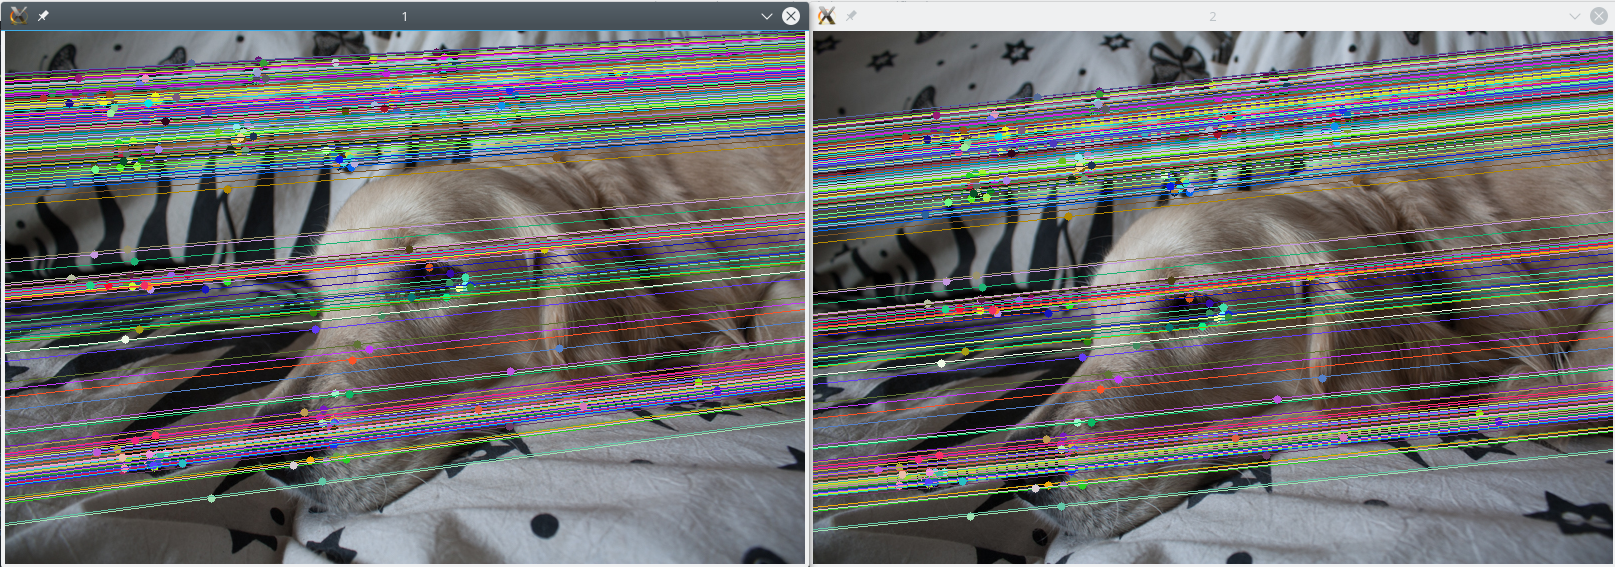
\includegraphics[width=160mm]{Lola-Normal.png}
    	\caption{Par original de fotografías de Lola, mascota de uno de los autores.}
    \end{figure}

    \begin{figure}[ht!]
        \centering
        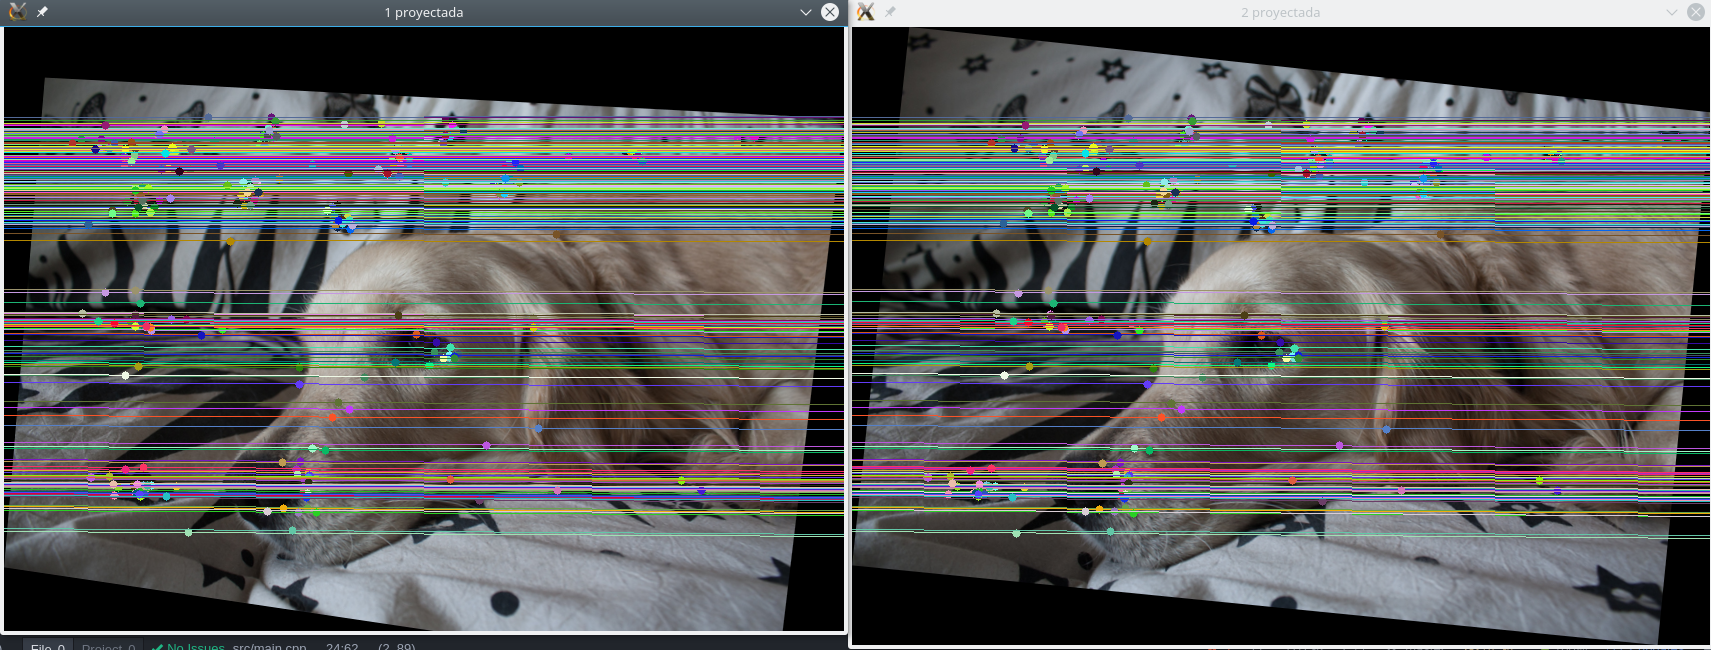
\includegraphics[width=160mm]{Lola-Proyectado.png}
        \caption{Par rectificado de fotografías de Lola, mascota de uno de los autores.}
    \end{figure}

    \begin{figure}[ht!]
        \centering
        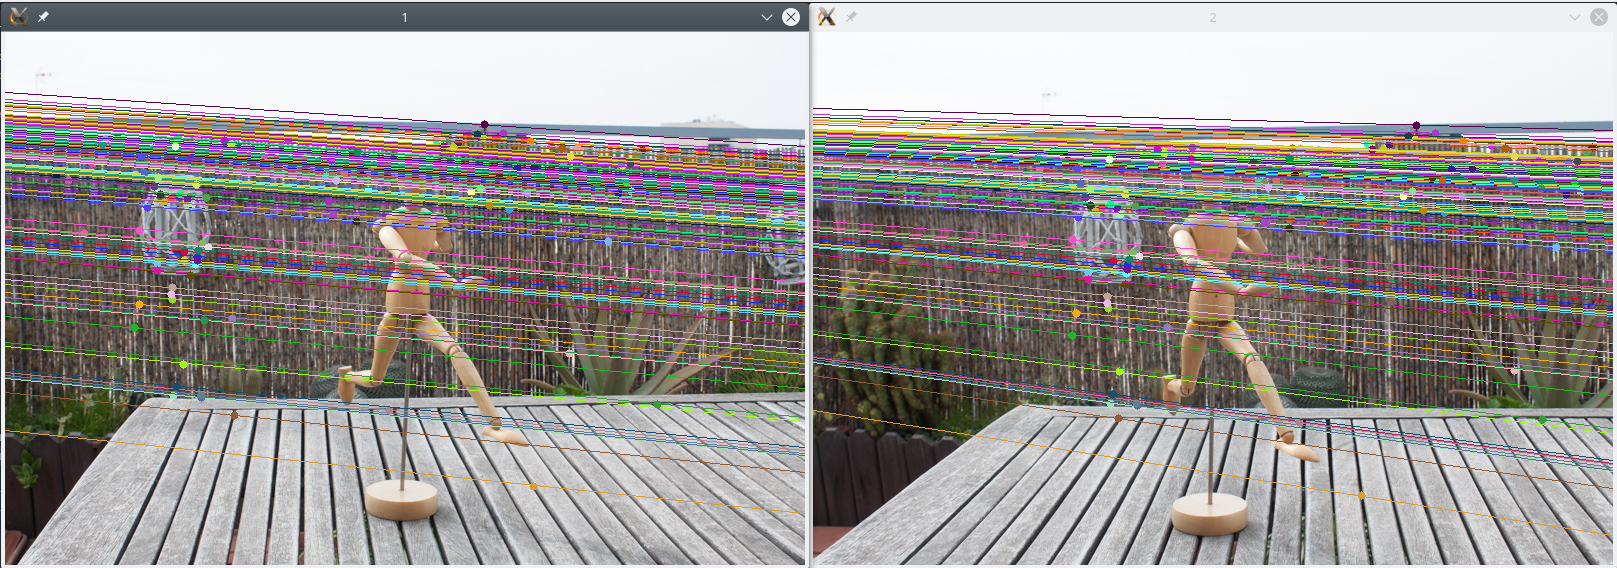
\includegraphics[width=160mm]{Monigote-Normal.png}
        \caption{Par original de fotografías de un muñeco de madera.}
    \end{figure}

    \begin{figure}[ht!]
        \centering
        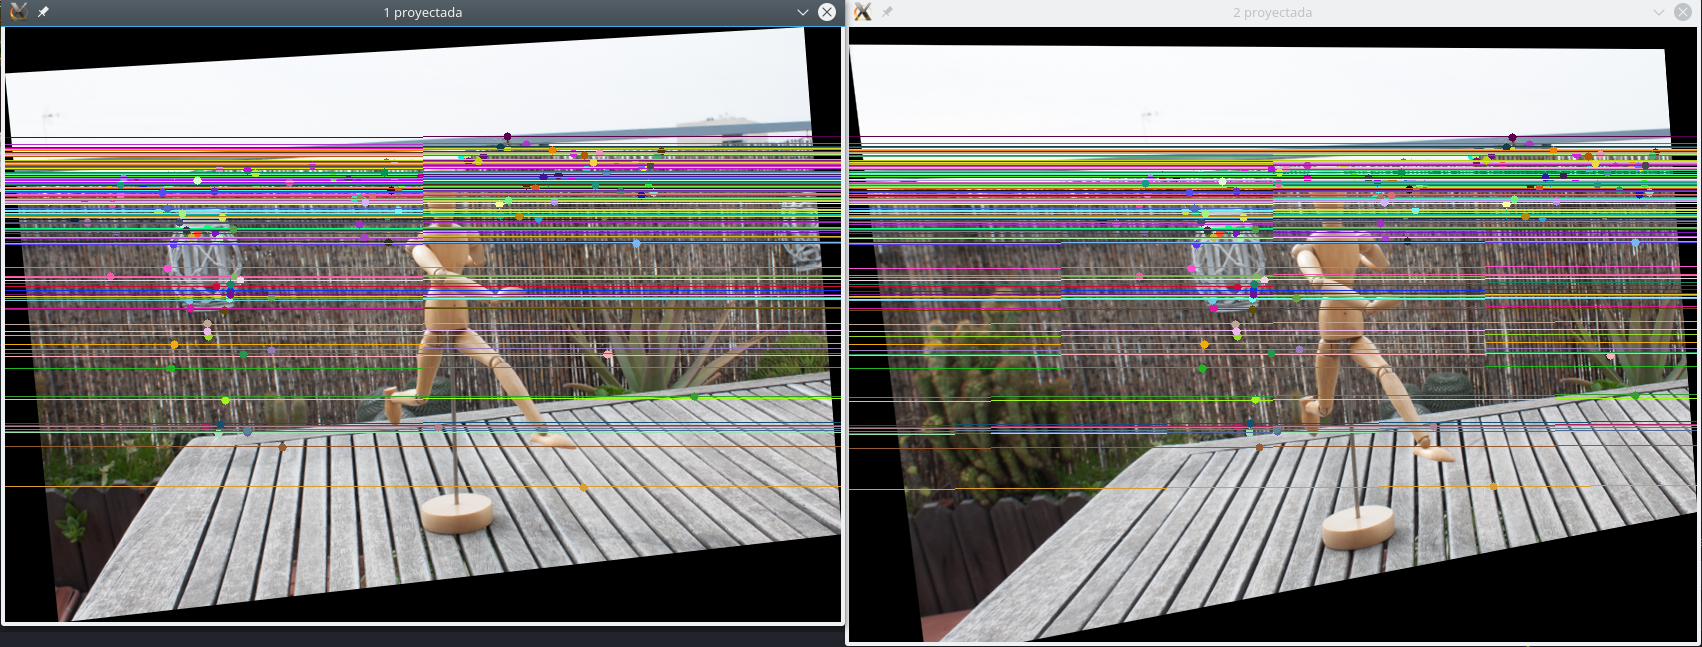
\includegraphics[width=160mm]{Monigote-Proyectado.png}
        \caption{Par rectificado de fotografías de un muñeco de madera.}
    \end{figure}

    \begin{figure}[ht!]
        \centering
        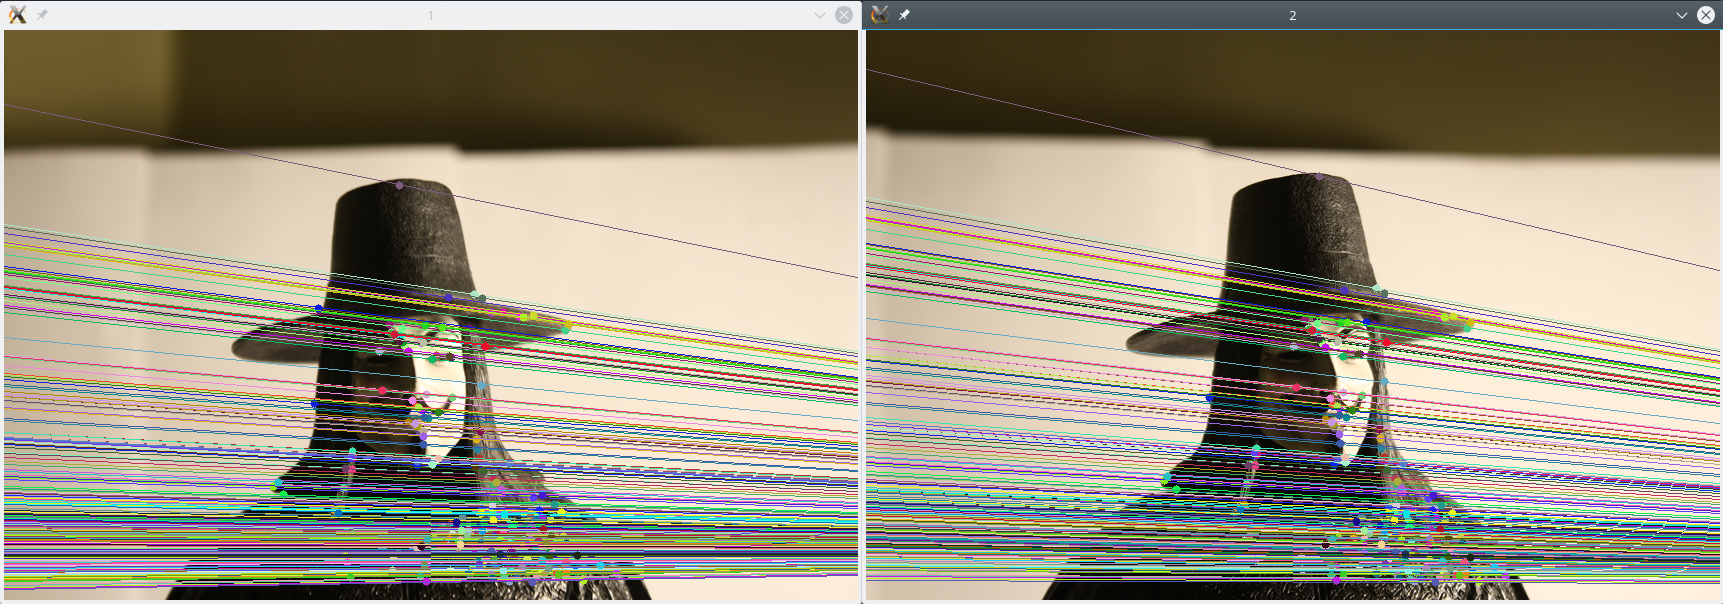
\includegraphics[width=160mm]{V-Normal.png}
        \caption{Par original de fotografías de una figura de cine.}
    \end{figure}

    \begin{figure}[ht!]
        \centering
        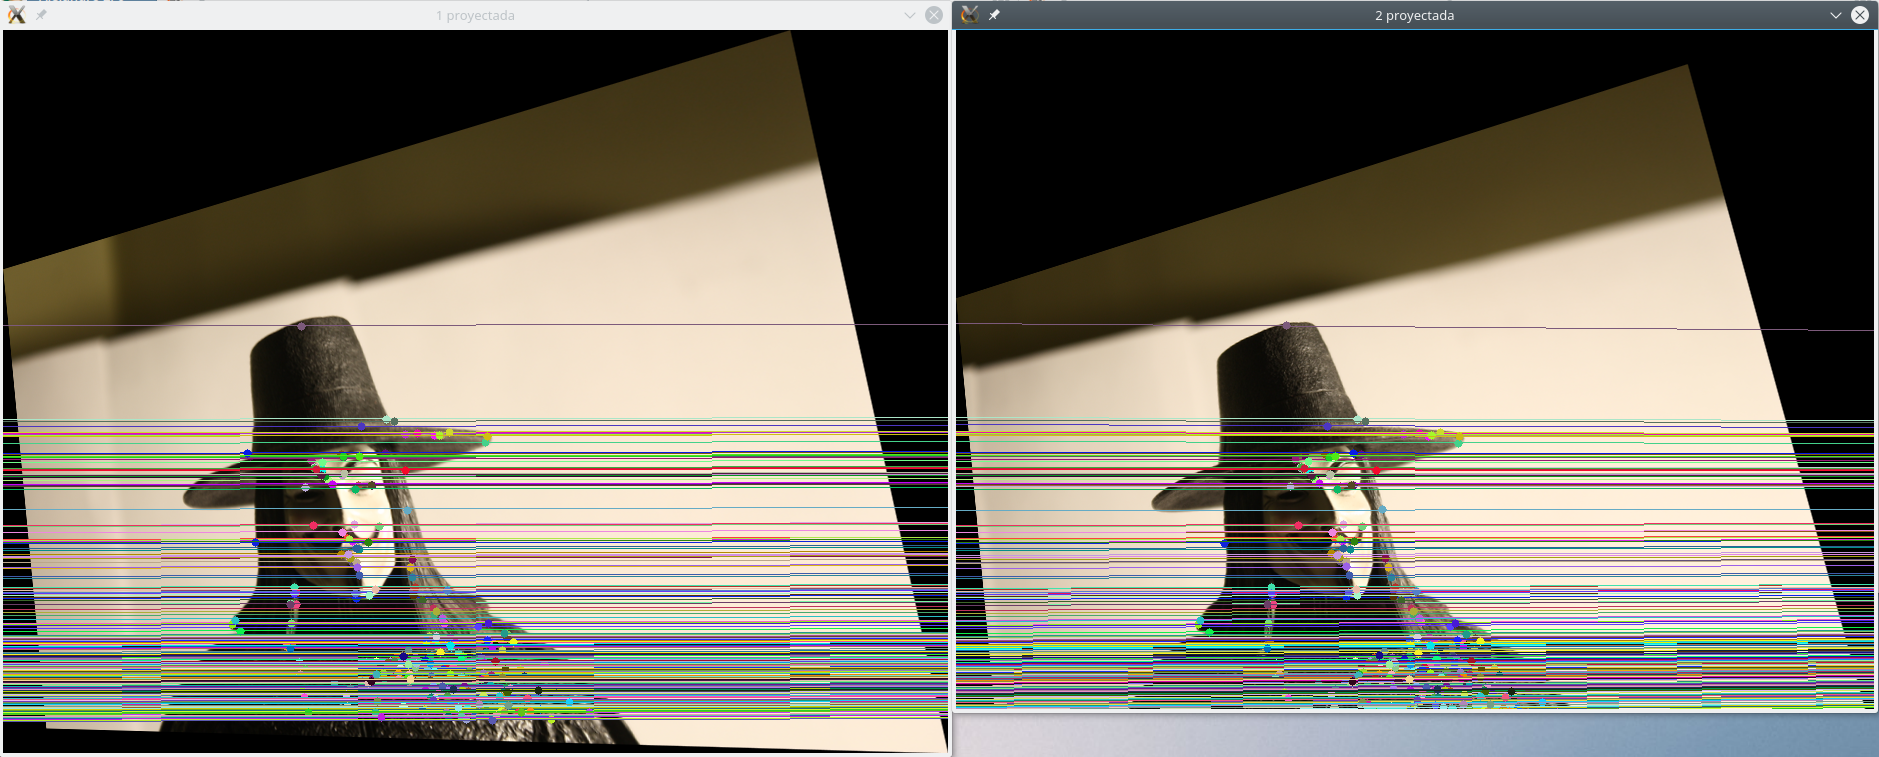
\includegraphics[width=160mm]{V-Proyectado.png}
        \caption{Par rectificado de fotografías de una figura de cine.}
    \end{figure}

    \clearpage
    \section{Valoración de resultados}

    Los resultado son, tanto visual como matemáticamente, tal y como se esperaban. Los epipolos, como se ve en las siguiente salidas, son tan cercanos al $[1, 0, 0]$ como la precisión de la máquina puede conseguir.

    En la ejecución se muestra el epipolo original normalizado por la tercera coordenada.

    En el par de imágenes de la perra, el epipolo original es $[5868.93, -278.987, 1]$ y el rectificado, $[0.999998, -0.002162, -1.76364e-05]$.

    En el par de imágenes del muñeco de madera, el epipolo original es $[-9167.01, -551.777, 1]$ y el rectificado, $[0.999999, -0.00146798, -2.12774e-06]$.

    En el par de imágenes del muñeco de cine, el epipolo original es $[2214.98, 523.468, 1]$ y el rectificado, $[0.999999, 0.00120902, 7.31557e-06]$.

    Visualmente, es claro que todas las líneas son horizontales, paralelas entre sí y están a la misma altura.

    En la ejecución del código se pueden ver los resultados de las comprobaciones matemáticas y de las homografías finales.


    % -------------------------- Bibliografía ------------------------
    \bibliographystyle{babplain}
    \bibliography{bibliografia}

\end{document}
